\documentclass[]{llncs}

\usepackage{graphicx}
\usepackage{algorithm}
\usepackage{algpseudocode}
\usepackage{float}

\begin{document}
\title{OPC UA based Smart Home} %titles have no end punctuation
\author{Yuankui Wang (Matr.-Nr.: 6670785)}
\institute{University of Paderborn \email{wangyk@mail.upb.de}}

\maketitle

\begin{abstract}

Object Linking and Embedding for Process Control Unified Architecture, knows as OPC UA is the most recent released industry standard from OPC Foundation, which compared with his predecessors is equipped with a list of charming new features, with whose help OPC UA is capable of solving imperfections that come along with OPC and offering more functionalities to the end users. In this paper, I will describe highlighting features of OPC Unified Architecture, especially focus on the security issues, analyze already well known attacks and corresponding countermeasures taken by OPC Unified Architecture, evaluate performance of different possible security polices and design a OPC UA standard based Smart Home to illustrate the implementation of essential parts of OPC Unified Architecture.  

\end{abstract}

\section{Introduction}

OPC from OPC Foundation has already found a great application area in today’s industry world, providing a set of standards used to support system interconnectivity and realize a common interface for communications between different products from different vendors. According to OPC Unified Architecture the future standard for communication and information modelling in automation from Wolfgang Mahnke, Stefan Leitner, there are over 22,000 products applying OPC offered by 3,200 vendors in automation industry.[1]


Even OPC standards are widely accepted, there exit still limitations. I.e. Most of all, OPC is windows platform dependent and based on Microsoft COM/DCOM technology, which is already deemphasized and shows less attraction compared with platform independent Web Services. Moreover although COM/DCOM should help OPC to conquer cross-computer distribution weakness, but it also brings several drawbacks. For instance, developer is not capable of controlling DCOM and has to face frequent DCOM configuration issues. [wiki] Also OPC only supports simple date type information and provides single hierarchy, which apparently is not able to meet increasing need from users. [2] And etc.
In order to solve all these imperfections, OPC Unified Architecture comes into the world, which is a radical update of OPC protocols and aimed to achieve simplicity, scalability, outstanding performance, perfect and flexible security, cross platform, always availability, robustness ,supporting complex date types.


In conclusion, OPC Unified Architecture is a platform independent industry policy, supports the secure communication based on different network conditions between client and server that are provided by various vendors. 





\section{OPC Unified Architecture Structure Overview }

\subsection{OPC UA Specification}

The whole OPC Unified Architecture specification is divided into three main parts, core specification parts, which consists of OPC UA concepts, security model, address space model, services, information model, service mapping and profiles, access type specification parts including date access, alarm and conditions, programs and historical access, at last utility specification parts covering discovery together with aggregates. 


In OPC Unified Architecture information that can be visited by clients is defined as address space [Spe1]and there is a set of services provided by OPC UA which are introduced in order to apply operations in the address space. The information in address space is organized as a set of in particular hierarchy structured objects. Clients can accept information provided by OPC Unified Architecture Servers in two major ways, binary structured data and XML documents, depending on the complexity of exchanged information, network quality and so on. In addition three kinds of transport protocol can be applied to support client server communication. They are: OPC UA TCP, HTTP/SOAP and HTTP. Also the hierarchy structure in which objects are organized in address space is also various according to OPC UA standards and not limited to simple single hierarchy.   


Another charming feature of OPC UA is Event Notifications. With the help of Event Notification, OPC UA servers are allowed to immediately after some conditions are satisfied publish data, which is subscribed by clients. In this way, clients can for instance discovery failures within client-server-communication quickly and recover as soon as possible, which in return minimizes the lost to the smallest possible amount and also they are able to observe the subscribed data more precisely and find the pink elephant as fast as possible.

\subsection{Secure Channel and Session}
Since some data exchanged between client and server could be extreme precious and should be protected from other malicious third party, OPC UA defines a full set of security model, with which developer of system can configure the security level of the application to meet the need of reality. With the security model, authentication of client and server, authorization, integrity and confidentiality of client-server- communication, auditability and availability of services are guaranteed. Also OPC UA provides a set of countermeasures against message flooding, eavesdropping, message spoofing message alteration, message reply, server profiling, session hijacking and so on[Spe2].
\begin{figure}
	\centering
	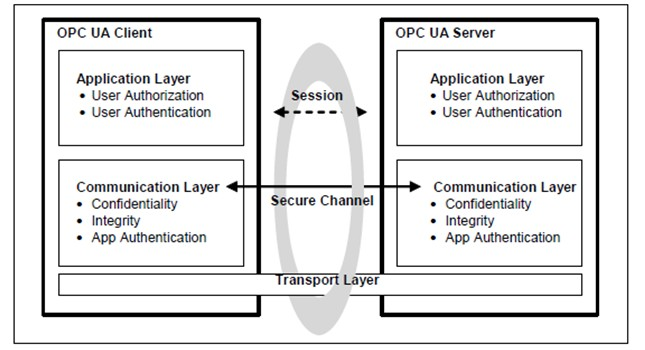
\includegraphics[width=0.75\textwidth]{opc_ua_cs_comm.jpg}
		\caption[ ]{OPC UA Client Server Communication}
	\label{fig:opc_ua_cs_comm}
\end{figure}


Figure~\ref{fig:opc_ua_cs_comm} [Spe4] pictures the typical security communication architecture of OPC UA. As shown in 1, the communication between OPC UA client and server is established above a secure channel, which is active during the whole application session. The secure channel is established only after successful validation of both client and server certificates and it provides necessary mechanisms to support confidentiality, message integrity and application authentication. On top of secure channel, is an application level session between OPC UA client and server, whose responsibilities are to transmit data information and commands. This session is also in charge of managing security policies like user authorization and authentication. It should be pointed out that, even a secure channel is out of work for some reasons, the session is still valid and OPC UA client and server involved in aforementioned session can still re-establish the broken secure channel. A secure transport layer is guaranteed by encryption and signatures defined by platform that support web services.

\subsubsection{Security Handshake}
Security handshake as below explains with some details about how secure channel and session are established.
\begin{figure}[!htb]
	\centering
	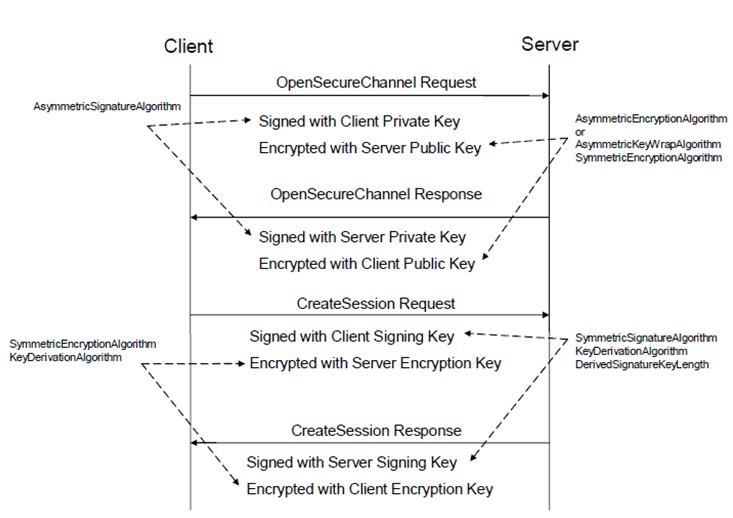
\includegraphics[width=0.75\textwidth]{opc_ua_shs.jpg}
		\caption[ ]{OPC UA Client Server Security Handshake}
	\label{fig:opc_ua_cs_shs}
\end{figure}

\subsubsection{OPC UA Client Server Communication Stack}
OPC UA client initiates the first OpenSecureChannel request and waits the response from server. Messages exchanged during the process of construction secure channel between client and server are encrypted using asymmetric encryption and signature algorithms. But some security protocols that could be applied according to OPC UA standard, are not using an asymmetric message encryption algorithm to encrypt to request/response messages. Instead, they apply AsymmetricKeyWrapAlgorithm to encrypt symmetric keys and use symmetric encryption algorithm with encrypted keys to encrypt messages. After a successful construction of secure channel, OPC UA client sends CreateSession request and waits for server response. Messages transported during this procedure are encrypted with symmetric encryption algorithms and signed with client/server signing key.

\begin{figure}[!htb]
	\centering
	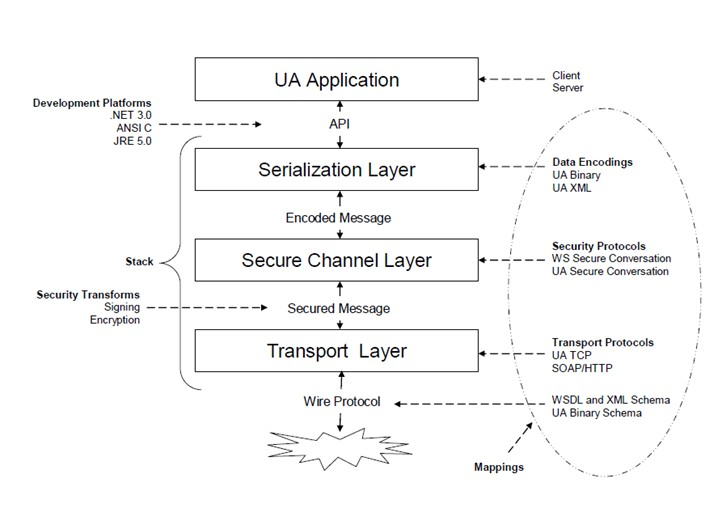
\includegraphics[width=0.75\textwidth]{opc_ua_commstack.jpg}
		\caption[ ]{OPC UA Client Server Communication Stack}
	\label{fig:opc_ua_commstack}
\end{figure}

\subsection{OPC UA Communication stack}

As discussed in subsection 2.2, the OPC UA communication stack is a three-layer architecture. Even the terminologies of those layers are defined as the ones used in ISO model, but layers in OPC UA are not directly equal to layers in ISO model. And figure x from OPC UA  6th specification gives a precise overview of each layer in OPC UA communication stack model, meanwhile it demonstrates functionalities performed by each layer. Serialization layer will divide long message into pieces referred as message chunk, and after then secure channel layer is going to encrypt each individual message chunk, not entire whole message. Likewise when receiving message chunk from others, OPC UA message receiver firstly verifies whether this message piece meets the security standard negotiated between OPC UA client and server. If not, this message receiver will close the secure channel. After a successful verification of all message chunks, the original OPC UA message will be reconstructed. Each secure message chunk applies the following structure.  

\begin{figure}
	\centering
	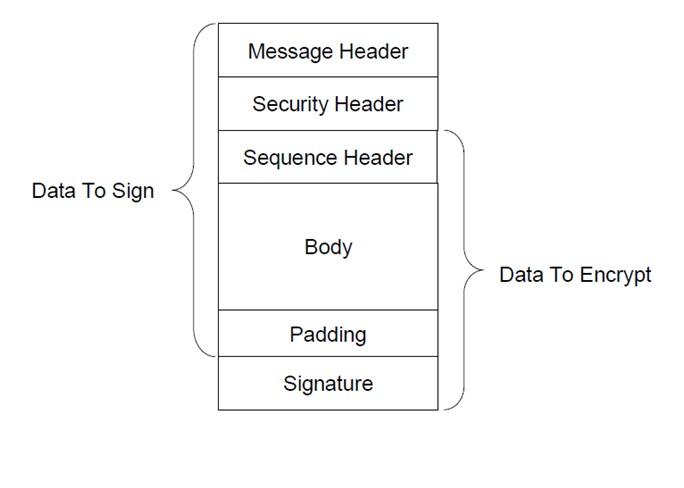
\includegraphics[width=0.75\textwidth]{opc_ua_messchunk.jpg}
		\caption[ ]{Message Chunk Structure}
	\label{fig:opc_ua_messchunk}
\end{figure}

In order to demonstrate, how OPC UA standards establish communication channel and build secure sessions, close message tunnel and reconstruc communication channel, it is assumed that the following demo OPC UA client and server set uses TCP/IP connection as transport layer protocol.

\begin{figure}[ht]
	\centering
	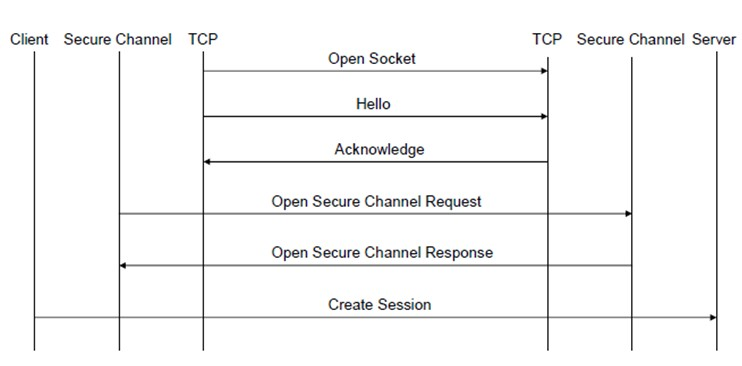
\includegraphics[width=0.75\textwidth]{tcp_1.jpg}
		\caption[ ]{Establish TCP/IP Connection}
	\label{fig:tcp_1}
\end{figure}
\subsubsection{Establishment of communication channel}
As the first step to create TCP/IP connection, this process is always initialized by OPC UA client. One OPC UA client initiates his socket and sends hello message, that includes buffer size which is supported and suggested by message sender, to the target OPC UA server. After receiving greeting message, OPC UA server answers the request for establishing TCP/IP connection with acknowledge message and sends information about supported buffer size, which is proposed by OPC UA client and defines the message chunk size used between this connection, to its secure channel. 
\begin{figure}[ht]
	\centering
	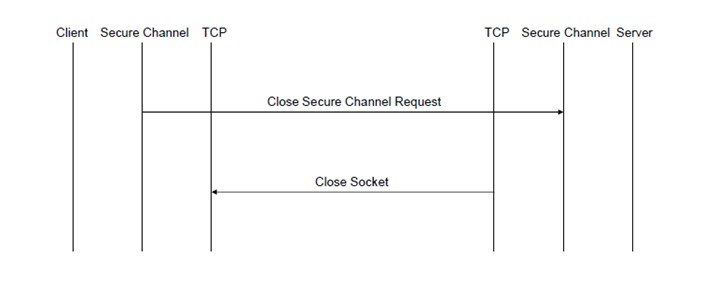
\includegraphics[width=0.75\textwidth]{tcp_2.jpg}
		\caption[ ]{Close TCP/IP Connection}
	\label{fig:tcp_2}
\end{figure}
\subsubsection{Close TCP/IP Connection}
This process is done when OPC UA server receives close secure channel request from OPC UA client.
\begin{figure}[ht]
	\centering
	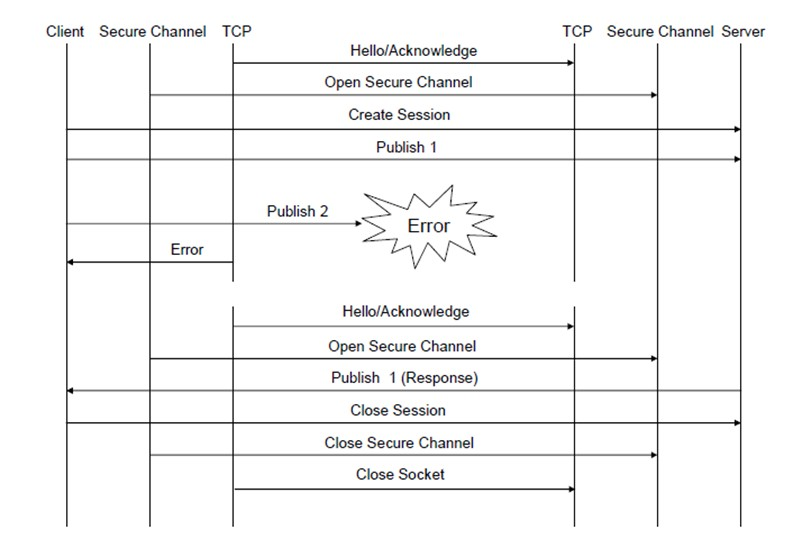
\includegraphics[width=0.75\textwidth]{tcp_3.jpg}
		\caption[ ]{Recover Secure Channel}
	\label{fig:tcp_3}
\end{figure}
\subsubsection{Recover Connection}


Whenever error occurs during TCP/IP connection between OPC UA client and server, client will try to periodically re-establish it until the session is closed or the lifetime of security token goes to an end. Also it should be pointed out that the buffer size defined by corrupt secure channel should not be changed during this error recover process.

\subsection{Historical Data}
Last but not least security feature offered by OPC Unified Architecture is auditing, which supports traceability of any behaviours occur in OPC UA system. That means any security related problem can be recorded and for future use.

\subsection{OPC UA client/ server structure}
\begin{figure}
	\centering
	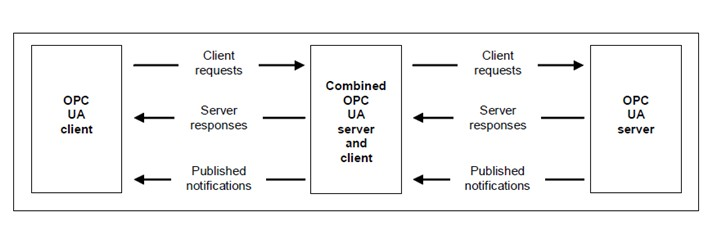
\includegraphics[width=0.75\textwidth]{cs.jpg}
		\caption[ ]{OPC UA Client Server Structure}
	\label{fig:cs}
\end{figure}
Figure 2 illustrates a typical OPC UA client server architecture and also describes a combined server-client. The routine communication between client and server consists of requests from client, corresponding responses sent from server and notifications which are generated because of client’s early subscription.

\begin{figure}
	\centering
	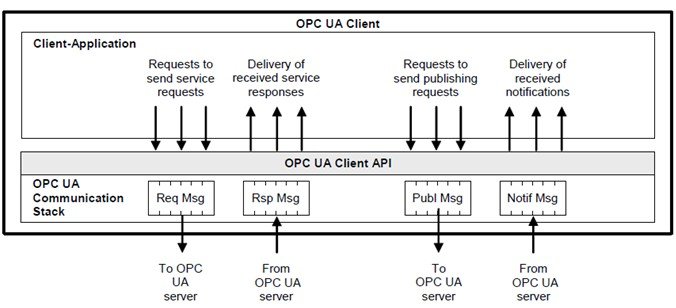
\includegraphics[width=0.75\textwidth]{client.jpg}
		\caption[ ]{OPC UA Client Structure}
	\label{fig:client}
\end{figure}

Figure 3 picture one simple OPC UA client containing client application, an internal API, isolating the application code from communication stack, and a communication stack that translates OPC UA client API calls.

\begin{figure}
	\centering
	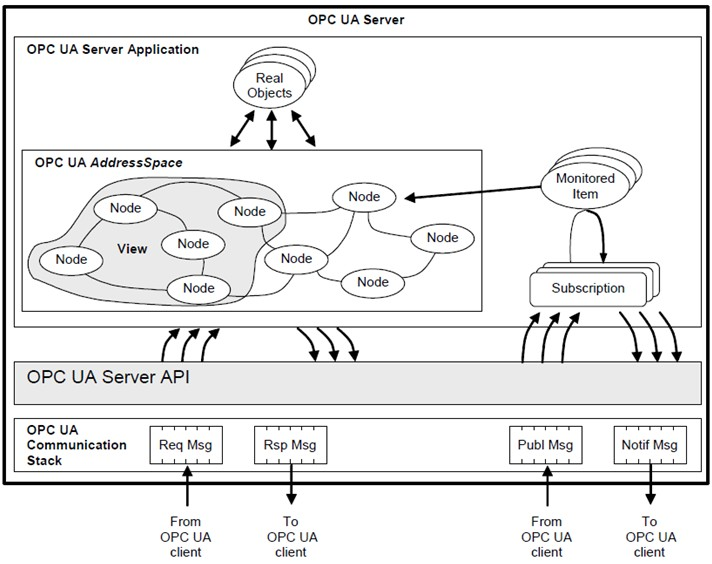
\includegraphics[width=0.75\textwidth]{server.jpg}
		\caption[ ]{OPC UA Server Structure}
	\label{fig:server}
\end{figure}
In figure 4, one OPC UA Server structure is explained. As the aforementioned client structure, it also includes three main parts, server application, internal API and communication stack. It is worth mentioning that, real objects here are referred as physical field devices or software application that is only maintained internally. View, which is pictured as a part of address space, presents nodes that can be browsed by clients

\subsection{Other Competitor}
WebSphere Message Broker Message Queuing Telemetry Transport (MQTT) is another machine to machine (M2M) communication protocol. Compared with OPC UA standard, MQTT also supports UDP protocol in the transport layer. In OPC UA, only unidirectional, client to server, communication is provided, but in MQTT server to client communication is also possible without server implements client code. Moreover the communication overhead of MQTT is in comparison with OPC UA is relative small. 


Even thought MQTT protocol supports communication environment with low bandwidth and high latency, OPC UA provides complex object model and supports more features, including historical data record, alarm, notification, complete security policies and this is reason why OPC UA is more suitable for the application scenario that handles sensitive data with complex structure and needs immediate response.


Another member from Internet of Things is Constrained Application Protocol  (CoAP) which is designed for the extreme simple electronic devices with less memory and computing power and original CoAP only runs over UDP. Compared with OPC UA, simplicity from CoAP is the advantage, but apparently it should be considered that in the implementation scenario other transport protocol could be used, like TCP, more functions and services other than pure message exchange between client and server, are requested from users.

\section{Implementation Scenario}
 \begin{figure}[!htbp]
	\centering
	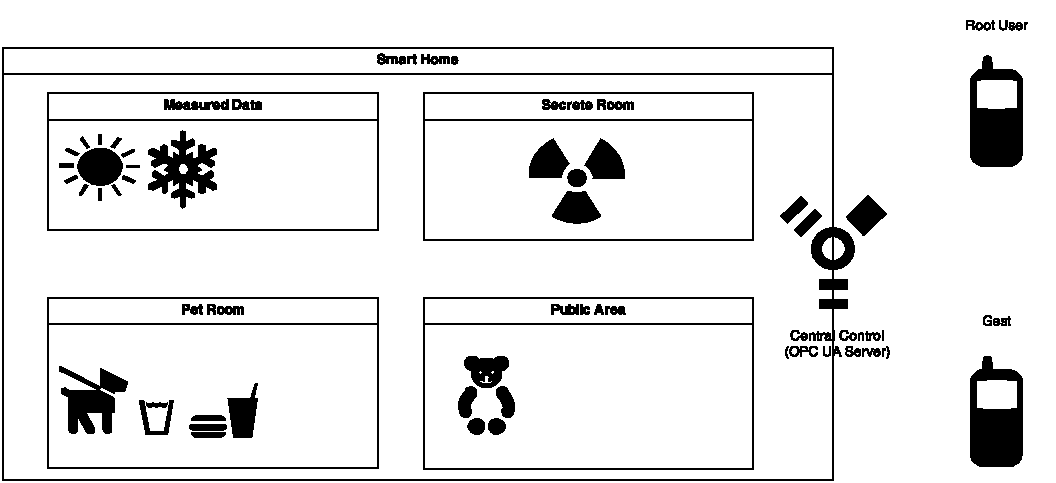
\includegraphics[width=0.75\textwidth]{SmartHome}
		\caption[ ]{Smart Home}
	\label{fig:SmartHome}
\end{figure}
Figure x describes the basic structure and functionalities of Smart Home. Central Controller also named as OPC UA Server is in charge of monitoring predefined environment variables, for instance, temperature, luminance and how much water the pet has, and taking corresponding behaviours, such as opening windows, turning off the heating or notifying pet owner that his/her puppy needs water. With the help of such services a more comfortable living condition is created in an automated way. Also OPC UA Server controls access right of entering each room, which means only authenticated users with enough authority can open the door. Moreover the root user, namely the owner of this house, is capable of assigning the permission of accessing particular room to other guests. In case of when he/she is taking a vocation and his/her pet cannot get the necessary care while he/she is away. At the same time, root user won’t worry about the person, who promises feeding pet, entries the forbidden room. At last, every single action taken by the OPC UA Server is recorded and is available for future use. 


In the implementation scenario, both OPC UA clients are Universal Integrated Circuit Car (UICC)  based handy user and OPC UA server is a computer with UICC card reader. Environment date is measured periodically by sensors and each room is locked, only the client, who is authenticated by server and holds enough authority can enter.
 \begin{figure}[ht]
	\centering
	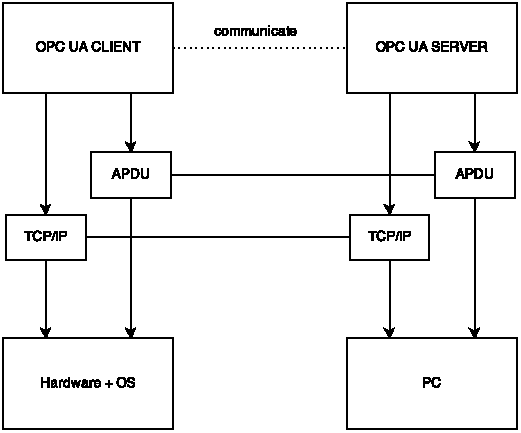
\includegraphics[width=0.75\textwidth]{softwareStructure}
		\caption[ ]{OPC UA Client Server Based On TCP/IP or APDU}
	\label{fig:softwareStructure}
\end{figure}
Figure x, describes possible software structure of aforementioned OPC UA client server structure. With different chip card, OPC UA client application is able to communicate with handy OS using Application Protocol Data Unit(APDU),which is a more nature way to exchange date between chip card and chip card application, or TCP/IP when Javacard 3 is applied.  
 \begin{figure}
	\centering
	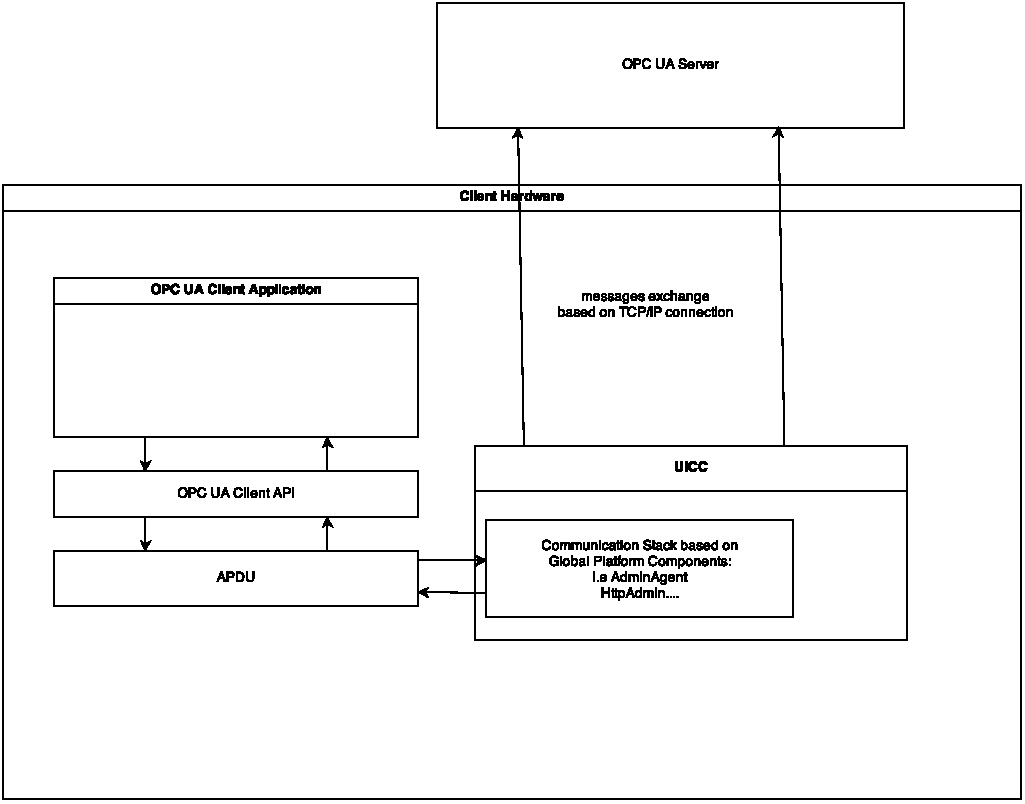
\includegraphics[width=0.75\textwidth]{clientStructure}
		\caption[ ]{Client Structure Using APDU}
	\label{fig:clientStructure}
\end{figure}
Based on the abovementioned application scenario, the basic architecture of OPC UA client is pictured as figure x when information exchanged between OPC UA client server application and chip card is in APDU format. OPC UA client is a smart phone with UICC card. OPC UA Client Application is build as a phone app. An OPC UA client API is the interface between application code and OPC UA communication stack, which is a Javacardapplet, that embedded on UICC chip card. The message that is exchanged between internal API and communication stack is in form of APDU. After receiving APDU from communication stack, UICC card will generate SMS submit and send this SMS to SMS server. SMS server will then forward this SMS to the OPC UA Server. Messages, such as OPC UA Server responds, notification information correspond to client subscriptions and OPC UA Server Acknowledgements are sent by SMS server and received by OPC UA client. Firstly SMS message is processed by CompacFormatCore integrated in UICC card and then forwarded to OPC UA communication stack. With the help of communication stack, messages from server are translated into APDU and sent to OPC UA server API, which will eventually pass them to OPC UA server application code. As OPC UA server is a gateway embedded with UICC card used.
 \begin{figure}
	\centering
	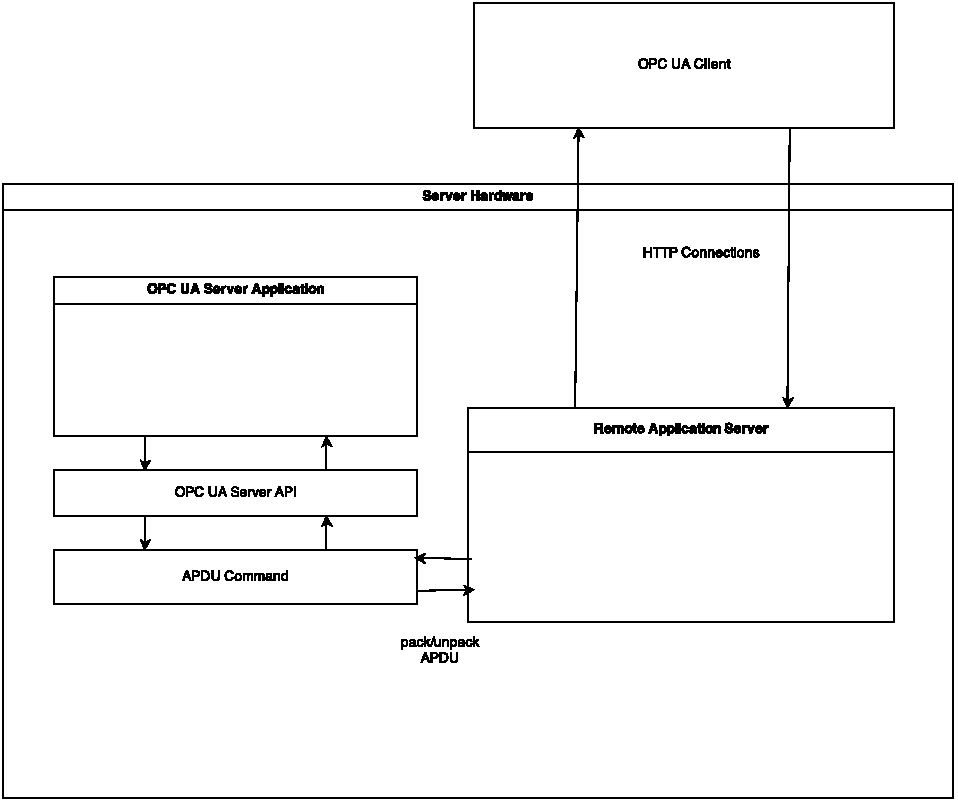
\includegraphics[width=0.75\textwidth]{serverStructure}
		\caption[ ]{Server Structure Using APDU}
	\label{fig:serverStructure}
\end{figure}

\section{Time Lines}
\begin{itemize}
  \item read paper, documentation, reference
  \item analyse and design communication stack that fits UICC card and meets OPC UA standard 
  \item design proto client/server structure 
  \item design models meeting OPC UA standards 
  \item analyse and design secure protocols. 
  \item design prototype
  \item programming
  \item debugging/performance analyse
\end{itemize}

\bibliographystyle{splncs}
\bibliography{wyk}
\end{document}
